%*----------- SLIDE -------------------------------------------------------------
\begin{frame}[t]{A problem} 
    \transdissolve[duration=0.5]
    Subsea pipe monitoring is an important application for the oil and gas industry to carry out \textbf{maintenance} that can \textbf{predict great damage} to the environment and monetary loss.

   
    %\newline
        \begin{columns}[t]
            
            \column{0.5\linewidth}
            \begin{center}
            \begin{figure}
                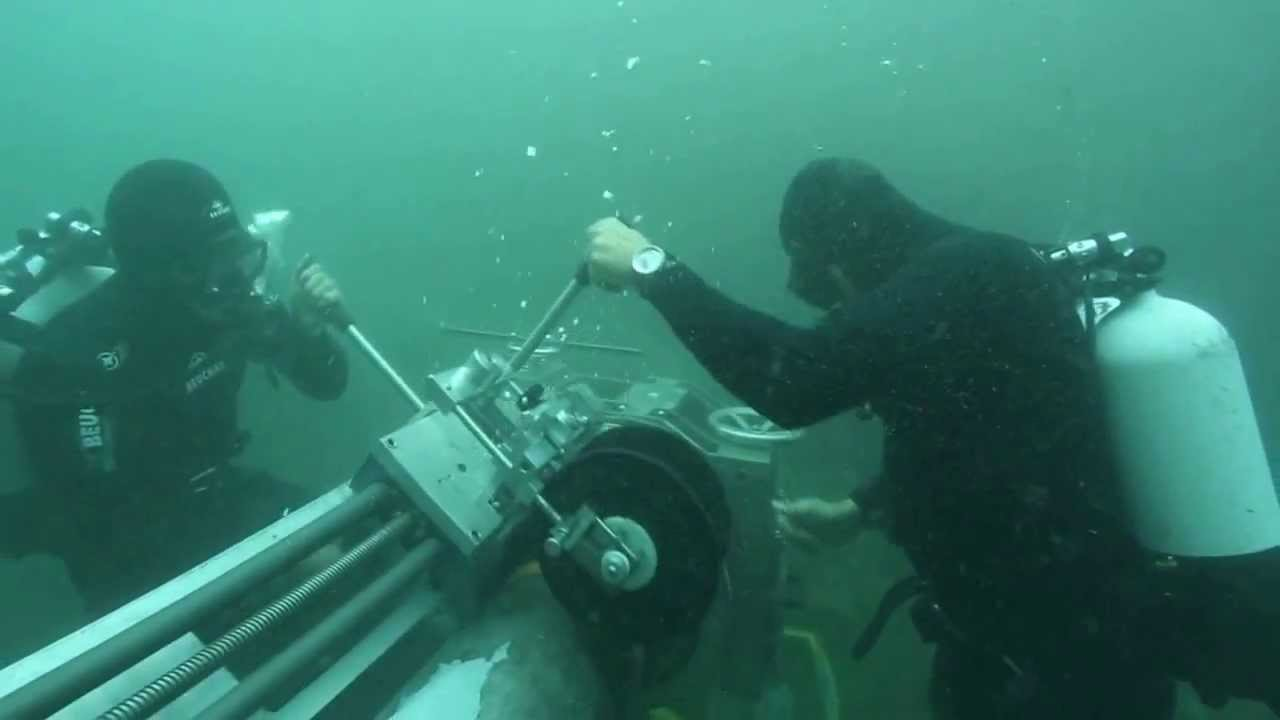
\includegraphics[width=0.8\textwidth]{man_pipeline.jpg}
               
               
                  
               
            \end{figure}

            \end{center}
            \column{.50\linewidth}
            %\vspace*{0.6cm}
            \begin{center}
          
                \begin{figure}
                    
                    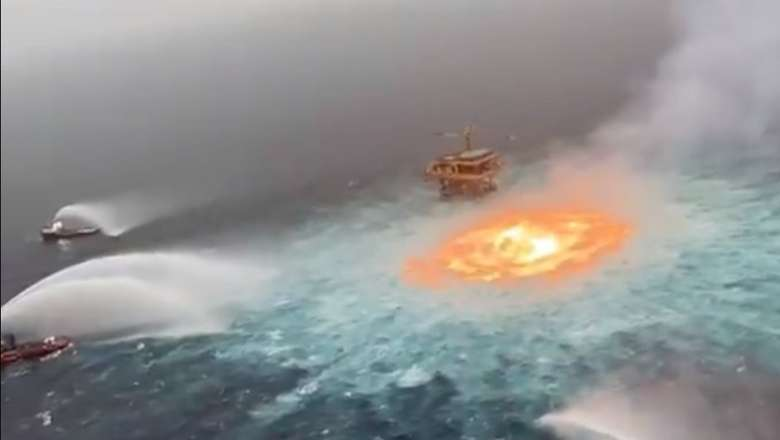
\includegraphics[width=0.8\textwidth]{leak.jpg}
                \end{figure}
            %}
            \end{center}
            
           
        \end{columns}
%*----------- notes
    \note[item]{Notes can help you to remember important information. Turn on the notes option.}
\end{frame}
%-
%*----------- SLIDE -------------------------------------------------------------
\begin{frame}[t]{A solution} 

    Underwater robotics are a good way to try solve this problem or at least minimize.



    \begin{center}
        \begin{figure}
            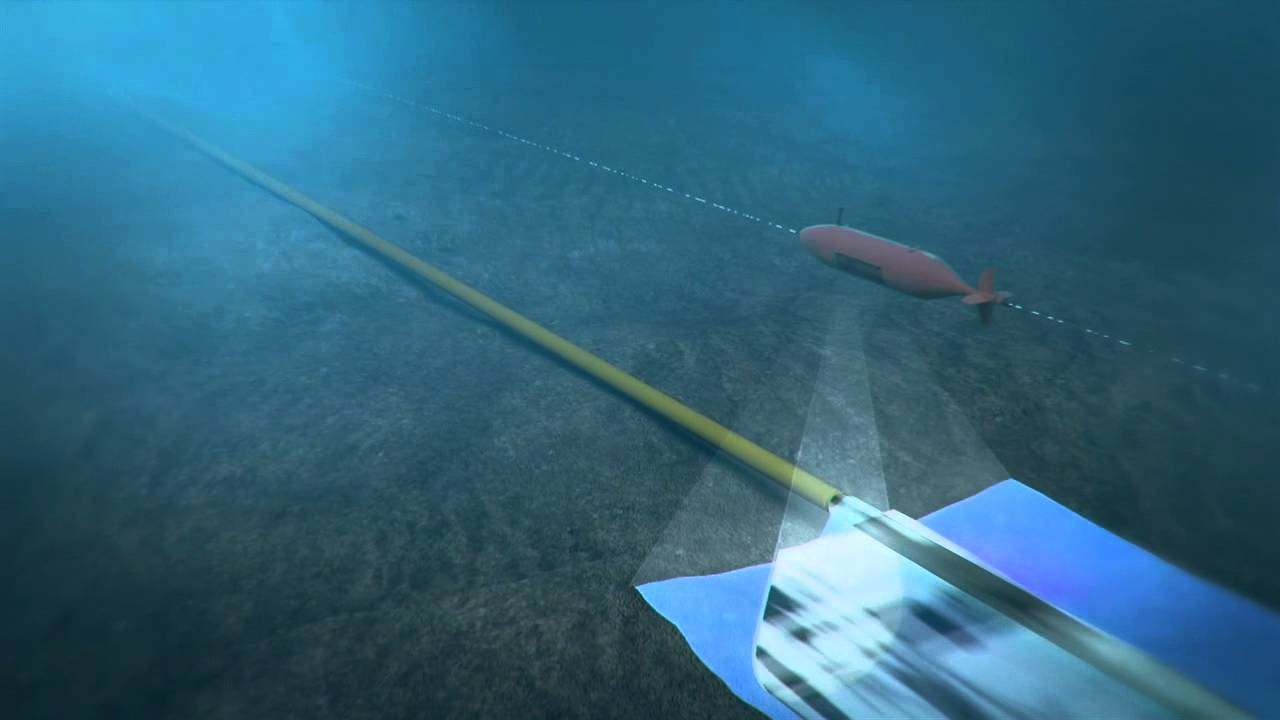
\includegraphics[width=0.65\textwidth]{inspection.jpg}               
           
        \end{figure}

        \end{center}
    
   % \transdissolve[duration=0.5]
   %
   % \begin{center}
   %     \Wider{%
   %     \begin{shaded}
   %     \begin{center}
   %         \vspace*{0.5cm}
   %         \resizebox{!}{0.5cm}{%
   %             \color{bg} The training of researchers in underwater robotics
   %         }%
   %     \end{center}
   %     \end{shaded}
   %     }%
   % \end{center}

\end{frame}


\begin{frame}{}
    \transdissolve[duration=0.5]
   
    \begin{center}
        \Wider{%
        \begin{shaded}
        \begin{center}
            \vspace*{0.5cm}
            \resizebox{!}{0.5cm}{%
                \color{bg} A Solution Equals A Challenge
            }%
        \end{center}
        \end{shaded}
        }%
    \end{center}
\end{frame}


\begin{frame}[t]{The Challenges} 
   The tasks the should be implement is operate a \textbf{pipe-following} using  underwater vehicle \textbf{BlueROV} in a simulation at Gazebo and \textbf{ROS2}.

   There are two challenges: \\
   \begin{itemize}

      \item A global
      \item A focused on underwater robotics field researchers
   \end{itemize}

   \begin{center}
    \begin{figure}
        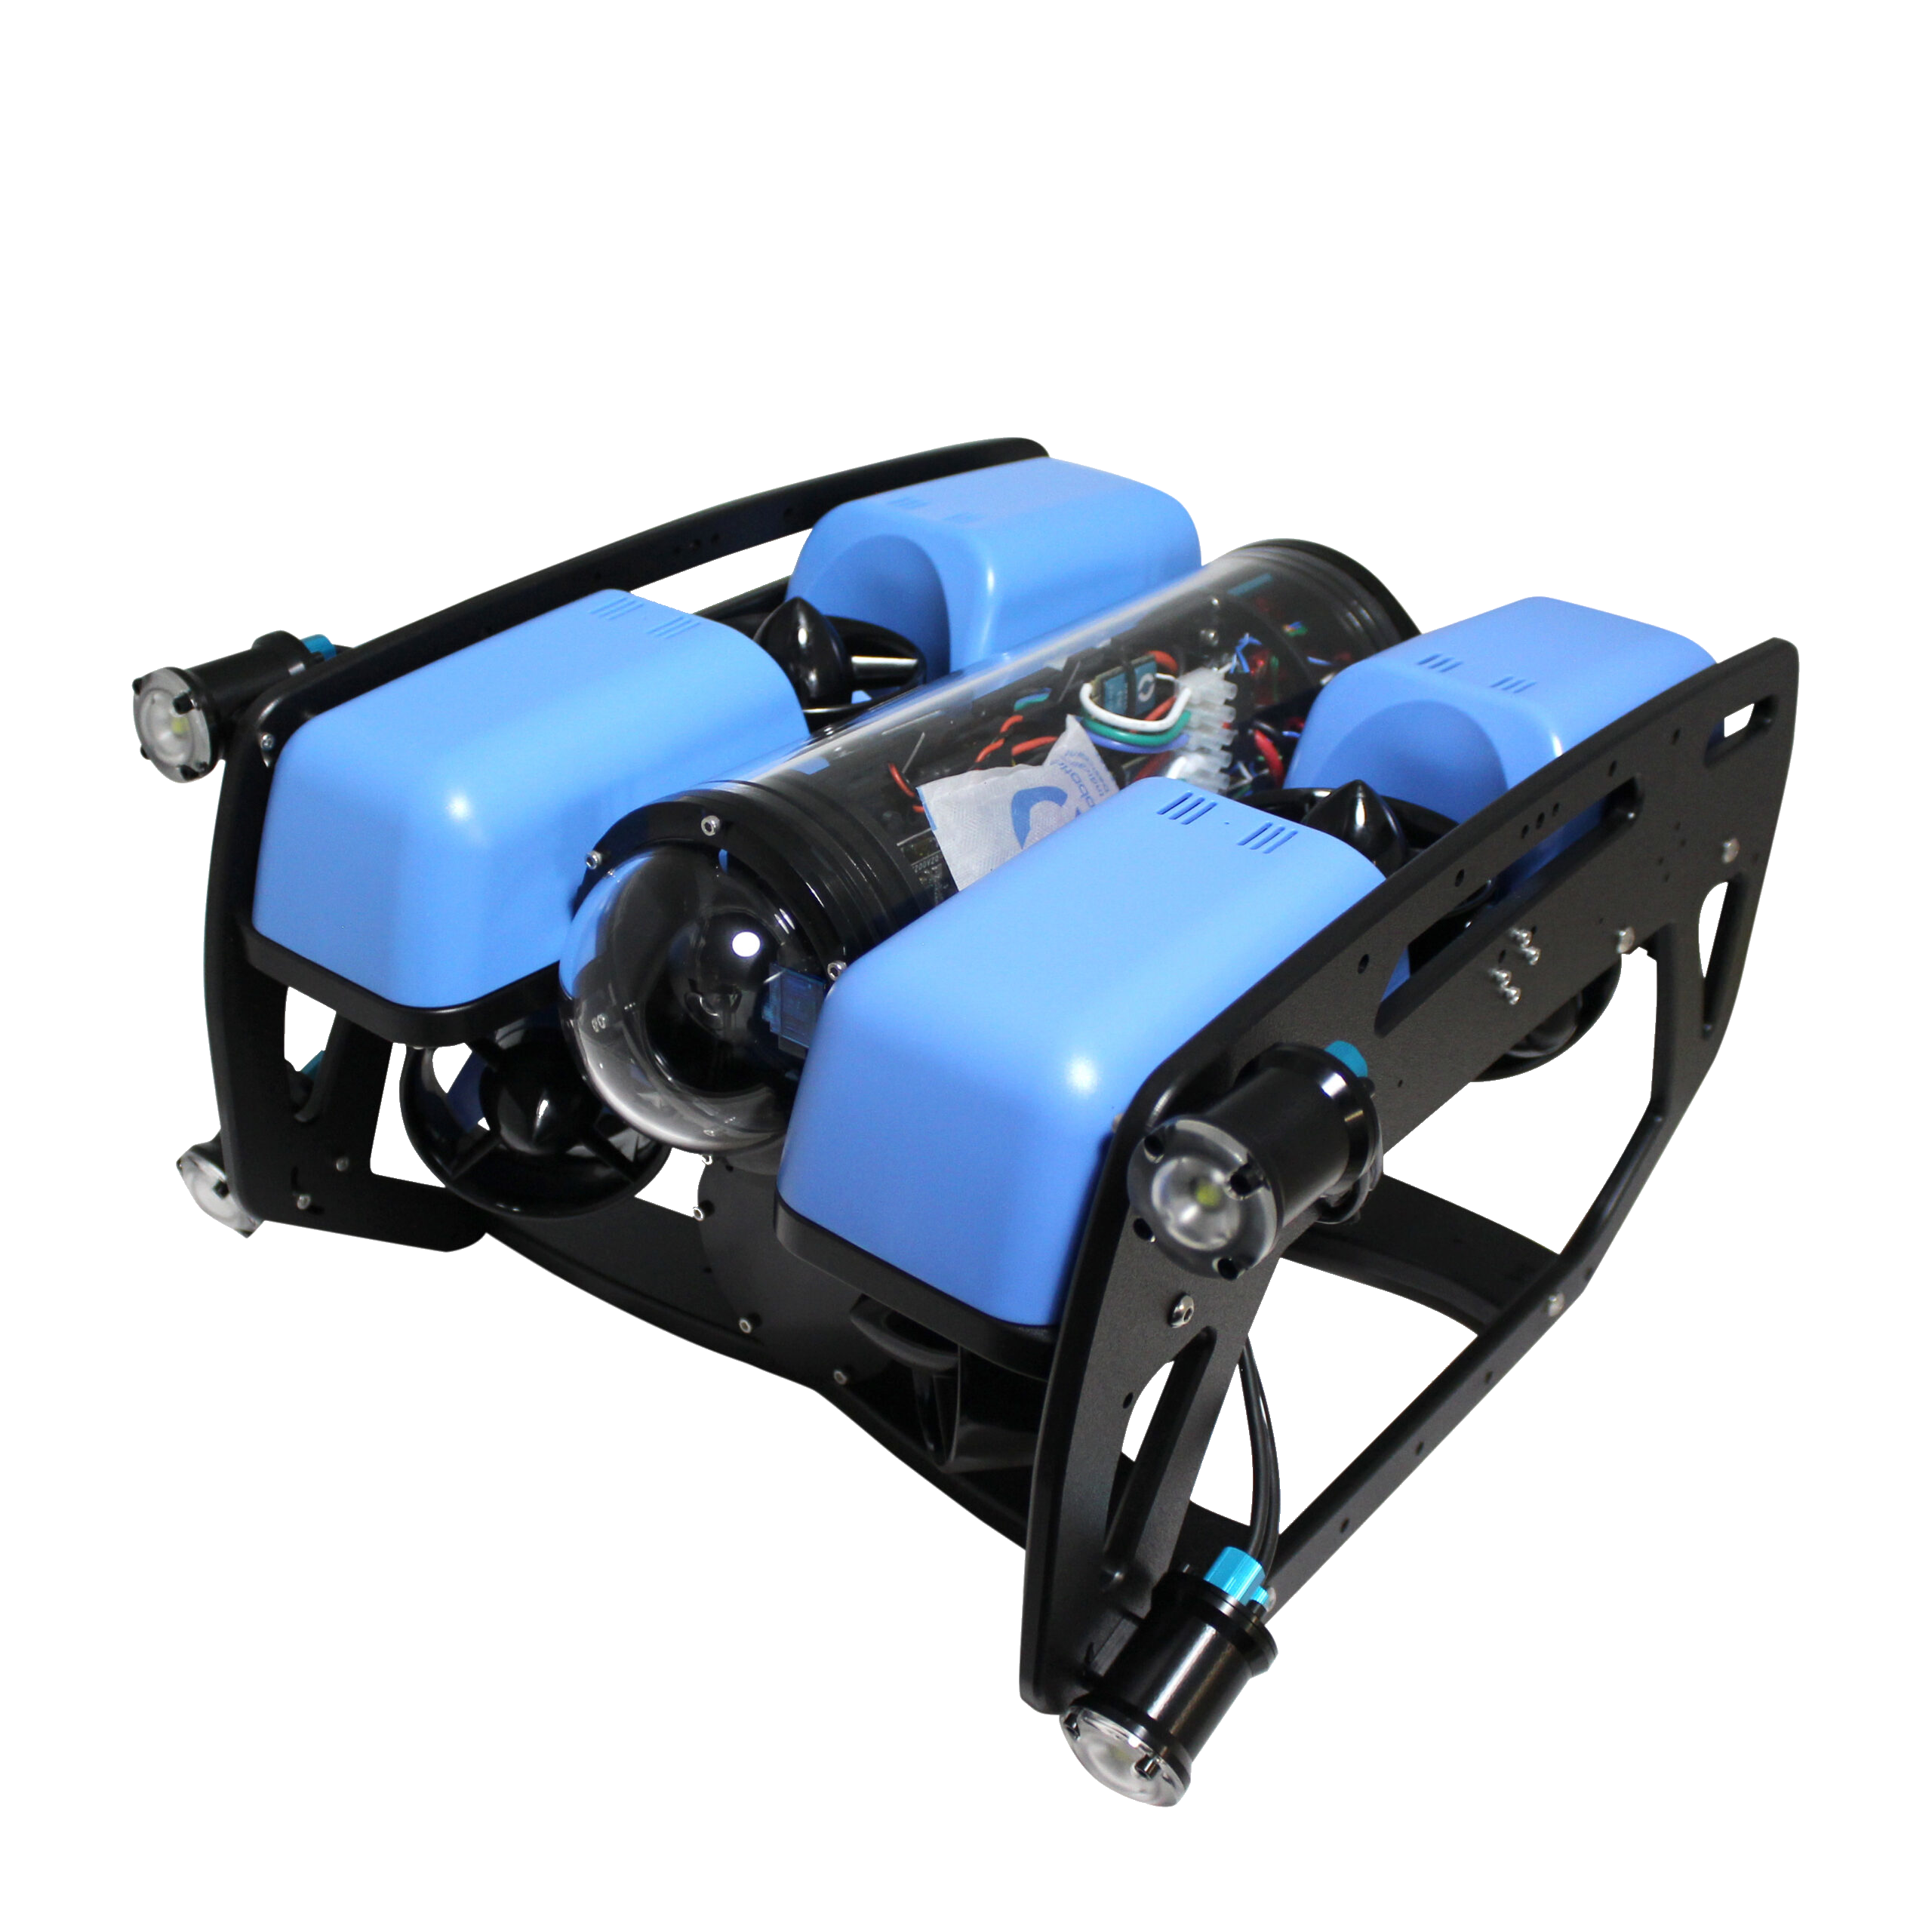
\includegraphics[width=0.30\textwidth]{bluerov.png}               
       
    \end{figure}

    \end{center}


\end{frame}


\begin{frame}{}
    \transdissolve[duration=0.5]
   
    \begin{center}
        \Wider{%
        \begin{shaded}
        \begin{center}
            \vspace*{0.5cm}
            \resizebox{!}{0.5cm}{%
                \color{bg} Global Challenge
            }%
        \end{center}
        \end{shaded}
        }%
    \end{center}
\end{frame}



\begin{frame}{}
    This challenge is broken down into \textbf{two stages}. The first execute the displacement of the vehicle from the initial point of the simulation to the initial pose of the identification of the pipe \textbf{autonomously}. The second is \textbf{monitoring the pipeline}. Artag will be placed at the initial and final point of identification



    \begin{center}
        \begin{figure}
            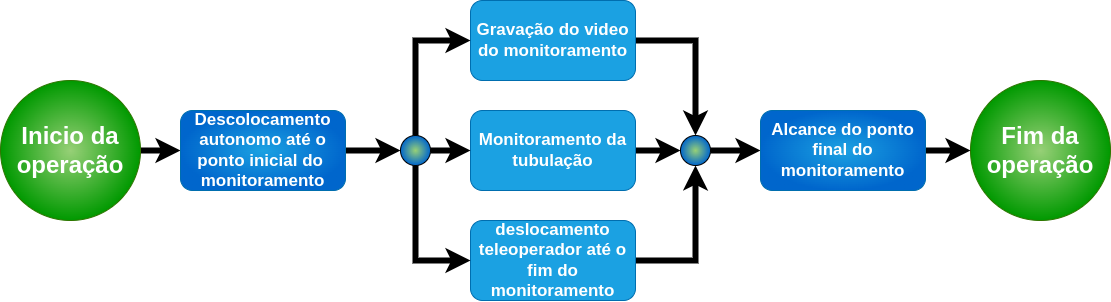
\includegraphics[width=0.8\textwidth]{global.png}               
           
        \end{figure}
    
        \end{center}
   
\end{frame}

\begin{frame}[t]{Minimal requirements}
    It is necessary to have:
    \begin{itemize}
        \item an intermediary knowledge in ROS
        \item C++ and/or Python
        \item Computer Vision
        \item Will
    \end{itemize} 


    \begin{columns}[c]
            
        \column{0.25\linewidth}

        \begin{center}
            \begin{figure}
                
\includegraphics[width=0.65\textwidth]{ros-logo.png}
            \end{figure}
        \end{end}

        \column{0.25\linewidth}

        \begin{center}
            \begin{figure}
                
\includegraphics[width=0.45\textwidth]{py.png}
            \end{figure}
        \end{end}

        \column{0.25\linewidth}

        \begin{center}
            \begin{figure}
                
\includegraphics[width=0.52\textwidth]{cpp.png}
            \end{figure}
        \end{end}


        \column{0.25\linewidth}
        \begin{center}
            \begin{figure}
                
\includegraphics[width=0.52\textwidth]{opencv.png}
        \end{figure}
    \end{end}

    \end{columns}
\end{frame}

\begin{frame}[t]{Gains}
    \begin{itemize}
        \item Hand on experiences on ROS2 and Gazebo
        \item developments Skills in coding
        \item Experience and knowledge with Computer Vision
        \item knowledge in underwater robotics
    \end{itemize}


    \begin{center}
        \begin{figure}
            
\includegraphics[width=0.3\textwidth]{reward.png}               
           
        \end{figure}
    
        \end{center}
   
\end{frame}

\begin{frame}{}
    \transdissolve[duration=0.5]
   
    \begin{center}
        \Wider{%
        \begin{shaded}
        \begin{center}
            \vspace*{0.5cm}
            \resizebox{!}{0.5cm}{%
                \color{bg} Field Challenge
            }%
        \end{center}
        \end{shaded}
        }%
    \end{center}
\end{frame}



\begin{frame}{}

    This Challenge has the objective of perform out the the \texbtf{pipeline follwing} 100\% \textbf{autonomously}. The vehicle must execute go-to-goal tasks to the initial point of pipeline and execute the \texbtf{pipeline follwing} \textbf{without human interference}.
   
    \begin{center}
        \begin{figure}
            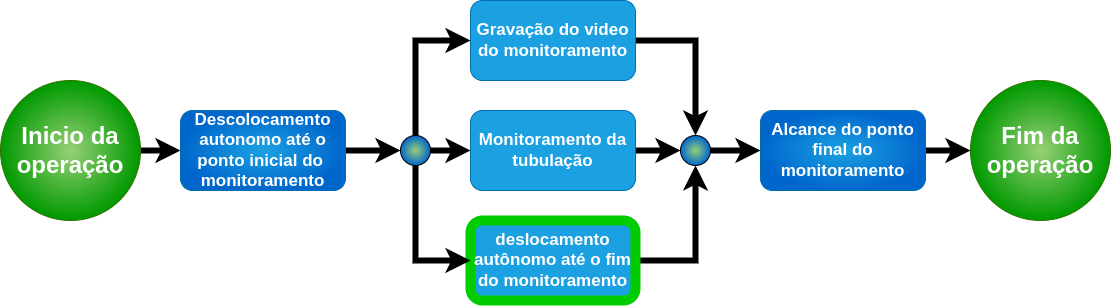
\includegraphics[width=0.8\textwidth]{filed.png}               
           
        \end{figure}
    
        \end{center}
\end{frame}

\begin{frame}{Minimal requiriments}
    It is necessary to have:
    \begin{itemize}
        \item an intermediary knowledge in ROS
        \item C++ and/or Python
        \item Computer Vision
        \item \textbf{Had realized the global challenge}
        \item Will
    \end{itemize} 

    \begin{columns}[c]
            
        \column{0.25\linewidth}

        \begin{center}
            \begin{figure}
                
\includegraphics[width=0.65\textwidth]{ros-logo.png}
            \end{figure}
        \end{end}

        \column{0.25\linewidth}

        \begin{center}
            \begin{figure}
                
\includegraphics[width=0.45\textwidth]{py.png}
            \end{figure}
        \end{end}

        \column{0.25\linewidth}

        \begin{center}
            \begin{figure}
                
\includegraphics[width=0.52\textwidth]{cpp.png}
            \end{figure}
        \end{end}


        \column{0.25\linewidth}
        \begin{center}
            \begin{figure}
                
\includegraphics[width=0.52\textwidth]{opencv.png}
        \end{figure}
    \end{end}

\end{columns}
   
\end{frame}

\begin{frame}[t]{Gains}
    \begin{itemize}
        \item Hand on experiences on ROS2 and Gazebo
        \item developments Skills in coding
        \item Experience and knowledge with Computer Vision
        \item knowledge in underwater robotics
            \item \textbf{Experience in executing a fully autonomous task in an underwater robot}
    \end{itemize}
    \begin{center}
        \begin{figure}
            
\includegraphics[width=0.3\textwidth]{reward.png}               
           
        \end{figure}
    
        \end{center}

    
   
\end{frame}


\begin{frame}{}
    \transdissolve[duration=0.5]
   
    \begin{center}
        \Wider{%
        \begin{shaded}
        \begin{center}
            \vspace*{0.5cm}
            \resizebox{!}{0.5cm}{%
                \color{bg} Are you ready?
            }%
        \end{center}
        \end{shaded}
        }%
    \end{center}
\end{frame}






    
   
